\chapter{Related works}
\label{ch:rel-works}

This chapter presents the related works we started from to develop this work. Firstly we introduce a paper from Laurenza et al. that explains how to build a malware triage framework for APT classification. The second work, from Caliskan et al., shows how is it possible to de-anonymize different programmers even with a compiled executable. The last work of Dubyk propose an approach for malware similarities based on the Rich Header.

\section{Malware Triage Based on Static Features and Public APT Reports}
Laurenza et al. show that it is possible to help an analyst lightening the number of samples to analyze, using a prioritization system \cite{laurenza2017malware}. 

They propose an architecture for sample prioritization, which, based on a rank score, decides which sample has the priority to be further inspected by an analyst. In this way, it is possible to avoid wasting time analyzing samples that are not important. 

They decide to rely only on static analysis instead of dynamic analysis to improve the speed of processing. In this architecture, the time elapsed for analyzing a classifying the samples is more important than the accuracy of the classification. Since it relies on static analysis, there is no need for sample execution, or to set up a complex virtualized environment. Every sample is processed, and some features are extracted from the header. The knowledge base created is used to classify new malware.

\begin{figure}
	\centering
	\begin{subfigure}{1.0\textwidth}
		\centering		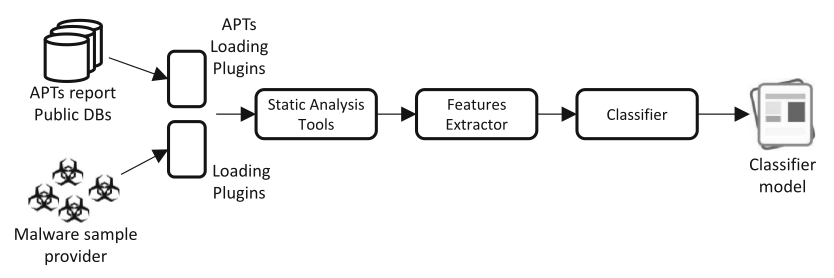
\includegraphics[width=1.0\linewidth]{train.png}  
		\caption{Training phase}
		\label{fig:sub-train}
	\end{subfigure}
	
	\begin{subfigure}{1.0\textwidth}
		\centering
		% include second image
		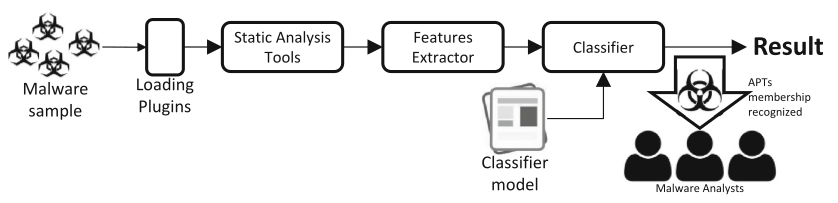
\includegraphics[width=1.0\linewidth]{test.png}  
		\caption{Testing phase}
		\label{fig:sub-test}
	\end{subfigure}
	
	\caption{Malware triage flow.}
	\label{fig:mal_triage}
\end{figure}

They propose a malware triage architecture, based on the identification of malware similar to other malware known to be related to some APTs campaign. The idea is to collect public APT reports and their related samples.  Then, extracting features from the samples and assigning them to the class of the APT they belong to. Those features vectors are used to train a classifier.

Figure \ref{fig:mal_triage} shows the architecture of both the training and testing phases. The APTs loading plugin frequently loads the information on APT crawled from public reports on the internet. The loading plugin feeds the system with new samples from different sources. The features extraction phase produces the features vectors from the malware, continuously updated by the previous loading plugin. In the classifier phase, a classifier is trained with features vector. 

In the analysis phase, novel samples follow the same pipeline; the features extraction stage extracts the features vector that is passed to the classifier. If the output of the classifier is positive, i.e., the sample is related a know APT, then the sample follows a different path, and is sent a human analyst for further inspection, otherwise it is discarded.

Unfortunately, this process has some drawbacks. First of all, it is possible to identify only samples correlated to a known APT campaign, if the sample belongs to a new never investigated APT, then it is impossible to detect it. Furthermore, even if the executable belongs to a known APT, there is no guarantee that the classifier detects it because it just relies on information present in the header of the file. The malware writer can hijack that information to mislead the model. 

Instead, deriving the features from the code analysis, and not only from the header, can mitigate this problem. However, it could still be possible to mislead the classifier modifying the code itself or using some code from other known APTs.

Sadly with our approach of using code analysis, the main problem is the dimensionality of the dataset. As we experienced, the number of features extracted can be huge, so feature selection is fundamental.




\subsection{dAPTaset}

Laurenza et al. have released \textbf{dAPTaset}, a public database that collects data related to APTs from existing public sources through a semi-automatic methodology and produces an exhaustive dataset \cite{daptaset}.

The database contains information about APT campaigns and their relation with public reports and samples. In our work, we are not interested in all the information contained in this database, but just a few of them. In particular, we need the relation between md5 of the file and APT campaign name. We extracted those columns from the database and saved in a \texttt{.csv} file for future use during features extraction.

The databes contains more than 2000 samples belonging to 15 different APTs: \textit{APT28,
APT29, APT30, Carbanak, Desert Falcon, Hurricane Panda, Lazarus Group, Mirage, Patchwork,
Sandwork, Shiqiang, Transparent Tribe, Violin Panda, Volatile Cedar, Winnti Group}.

Unfortunately, the dataset is not big enough and is not perfectly balanced, due to the nature of APT. It contains only 2086 samples because there are not many malware belonging to an APT campaign. Instead, the majority of public analyzed executable are just malware.

\section{De-anonymizing Programmers from Executable Binaries}
In this paper, Caliskan et al. presented their approach to de-anonymize different programmers from their compiled programs \cite{caliskan2015anonymizing}. They used a dataset of executables from Google Code Jam, and they show that even after compilation the author fingerprints persist in the code, and it is still possible to de-anonymize them.

Their paper is an entry point for our work, and we tried to apply the same approach to the APT triage problem. Their approach was to extract distinct blocks of features with different tools and then analyze them to determine the best ones to describe the stylistic fingerprint of the authors precisely. Firstly,  with a disassembler is possible to disassemble the binary and to obtain the low-level features in \textit{assembly} code.

Then with a decompiler, they extracted the \textit{Control Flow Graph} and the \textit{Abstract Syntax Tree}. Using the \textit{CFG}, the \textit{AST}, and the \textit{disassembled code} they derived the features set.

For this purpose, they used \textbf{ndisasm} for disassembling the binaries. Then using \textbf{radare2}, they generated the \textit{Control Flow Graph}. They used \textbf{Hexrey decompiler} for decompiling the executables and generating their source code. Lastly they used \textbf{Joern}, a C fuzzy parser, to parse the output of \textbf{Hexrey decompiler} and to produce the \textit{Abstract Syntax Tree}.

They used different types of feature selection techniques, such as WEKA's information gain, to reduce the number of features to only 53. They trained a \textit{RandomForestClassifier} with the dataset created to de-anonymize the authors correctly.

However, the tools used by Caliskan et al. are outdated and no more maintained, so we decided to use the novel open-source tool Ghidra to write the script and extract the information we want. In this way, we significantly reduced the amount of time for feature extraction.



\section{Rich Header}

Maksim Dubyk \cite{dubyk2019sans} shows how the rich header produces a robust series of data points that can be exploited in static PE-based malware detection. The Rich Header is an undocumented section of \textit{Portable Executable} (\textbf{PE}) header and provides a view of the environment where the executable was built. Firstly, Dubik shows the location of the Rich Header, how to understand and decrypt it, and how to extract it. Then, he shows different techniques to leverage the header for PE-based malware classification. The Rich Header is part of our features vector.

When building a PE, there are two distinct phases. The first one is the \textit{compilation phase}, where the high-level instructions from programming language are compiled into machine code, executable by the computer. The second one is the \textit{linking phase}, a combination of those different machine code objects into a single executable. The act of combining different objects creates the Rich Header. However, only executables compiled with Microsoft Linker contain the rich header. Other compilers, such as gcc or .Net,  do not have it.

\begin{figure}[!h]
	\centering
	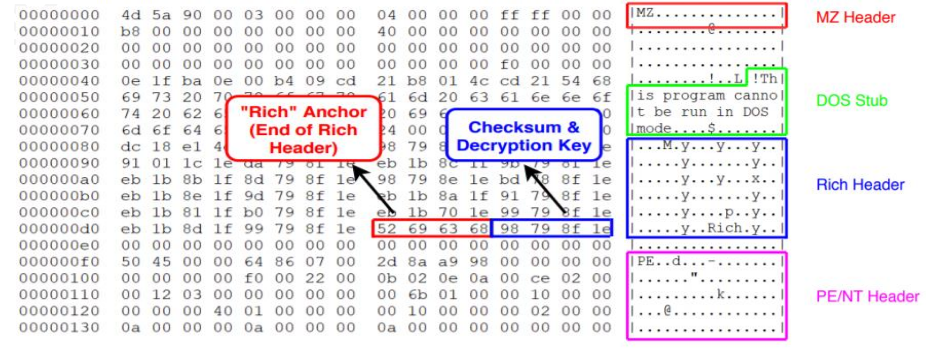
\includegraphics[width=1.0\columnwidth]{cmd.png}
	\caption{Hexview of cmd.exe}
	\label{fig:cmd}
\end{figure}

Analyzing an executable with a hexdump, the Rich Header starts from location \texttt{0x80} until the bytes sequence \texttt{0x52696368}, which means \textbf{"Rich"} in ASCII. Figure \ref{fig:cmd} shows the location of Rich header and the ending string "Rich". The content of the rich header is encrypted, and the corresponding decryption key and checksum are located right after the "Rich" string. 

The algorithm that computes the decryption key takes advantage of two checksum algorithms. The first checksum is generated from the bytes that make the DOS header, but with the \texttt{e\_lfanew} field zeroed out\cite{richHeaderHunting}. The second checksum is the combination of each value in the array generated. The outputs of the checksum algorithms are summed together and then masked with the bytes \texttt{0xFFFFFFF}, the key generated is then used to encrypt the rich header section using the XOR.

It is straightforward to decrypt the rich header section. The key found after the "Rich" string is XORed backward with the chunks of the section until the end string "DanS" is found.  

The decrypted rich header is an array that stores metadata related to each phase of the linking process. Each array's element is an 8-byte structure that contains three fields: \textit{product identification} (\textbf{pID}), \textit{product version} (\textbf{pV}), and a \textit{product count} (\textbf{pC}). Those numbers identify the Microsoft product used in that linking phase. However, since the Rich Header is an undocumented section, there is no official mapping of pID with Microsoft products. Nevertheless, some researches partially mapped out some pID with known compilers \cite{richGit}.

To calculate the rich header of each sample, we used the python script provided in \cite{dubyk2019sans}.